
\documentclass[aspectratio=1610]{beamer}

\usepackage[english]{babel}
\usepackage[utf8]{inputenc}
\usepackage[T1]{fontenc}

\usepackage{lmodern}
\usepackage{amsmath,amsfonts,amssymb}

\usepackage{graphicx}
\usepackage{pgf}



\usepackage[backend=biber, citestyle=authortitle-comp, bibstyle=authortitle]{biblatex}
\usepackage{csquotes}
\renewcommand{\bibliography}[1]{} % make noop. stillincl this cmd for
\bibliography{../techdoc/bib/bibi}           % texnicenter to display the library
\addbibresource{../techdoc/bib/bibi.bib}
%\bibhang1.5em 


%\usepackage[pdftex]{hyperref} %import last!
%\hypersetup{pdftex}
\usepackage{pgf}
%\usepackage{pgfmath}
\usepackage{pgffor}
\usepackage{ifthen}
\newcommand{\ani}[3]{
  \foreach \i [count=\ni] in {#2, ..., #3} {%
    \ifthenelse{\i=#2}{%
      \imgframe{\i}{#1}%
    }{\ifthenelse{\i=#3} {
      \imgframe{\i}{#1}%
    }{
      \imgframe[\transduration{0.1}]{\i}{#1}%
    }}%
  }%
}

\newcommand{\imgframe}[3][]{
  \begin{frame}
    #1
    \makebox[\linewidth]{\parbox{17cm}{
    %\frametitle{Frame #2}
      %\includegraphics[width=\paperwidth]{#3#2}
      \includegraphics[width=17cm]{#3#2}
    }}
  \end{frame}
}




\usepackage{appendixnumberbeamer}

\usetheme{Antibes}
%\usecolortheme{lily}
%\usefonttheme{professionalfonts}
\useinnertheme{default}
\useoutertheme{default}

\setbeamercovered{transparent}

% switch of nav
%\beamertemplatenavigationsymbolsempty

%frame number
\setbeamertemplate{footline}[frame number]

\mode<presentation>

\title{SpagthettiLens}
\subtitle{Gravitational Lens Modeling}
\author[R. Küng]{Rafael Küng}
\institute[ITP -- UZH]{Institute for Theoretical Physics\\ University Zurich}
\date[26.09.13]{26. Sept 2013}
%\logo{\pgfimage[width=3cm]{imgs/uzh}}
\titlegraphic{\includegraphics[width=4cm]{imgs/uzh}}
\subject{Modeling}
\keywords{ART, Gravitational Lens, Model, Modeling}


\begin{document}
{
\setbeamertemplate{logo}{}
\begin{frame}
	\titlepage
\end{frame}
}

\section*{Outline}

\begin{frame}
  %\frametitle{Inhaltsverzeichnis}
  \tableofcontents%[pausesections]
\end{frame}


\section*{Motivation}

\section{Theory}

\subsection{Fermat’s Principle}

\begin{frame}
  \frametitle{Fermat’s Principle}
  \begin{block}{Fermat’s Principle}
    Time $t$ for path $X$:
    $$t\left[X\right] = \frac{1}{c}\int_{t_1}^{t_2}n\left(\vec{x}\left(t\right)\right)\sqrt{1+\left(\frac{\text{d}\vec{x}\left(t'\right)}{\text{d}t'}\right)^2}\text{d}t'$$
    Path $X$ where $t$ stationary.
  \end{block}
\end{frame}

\ani{ani/1/n1-}{1}{45}
\ani{ani/1/n2-}{45}{50}

\subsection{ART}

\ani{ani/2/n1-}{1}{42}
\ani{ani/2/n2-}{41}{47}
\ani{ani/2/n3-}{46}{50}

\begin{frame}
  \frametitle{ART}
  \begin{block}{Field Equations}
    $$R_{\mu\nu} - \frac{R}{2}\, g_{\mu\nu} + \Lambda\, g_{\mu\nu} = \frac{8 \pi G}{c^4}\, T_{\mu\nu}$$
  \end{block}
\end{frame}


\subsection{Arrival Time Surface}

{\setbeamertemplate{tree}{}
\begin{frame}
  
  \hspace{-1.2cm}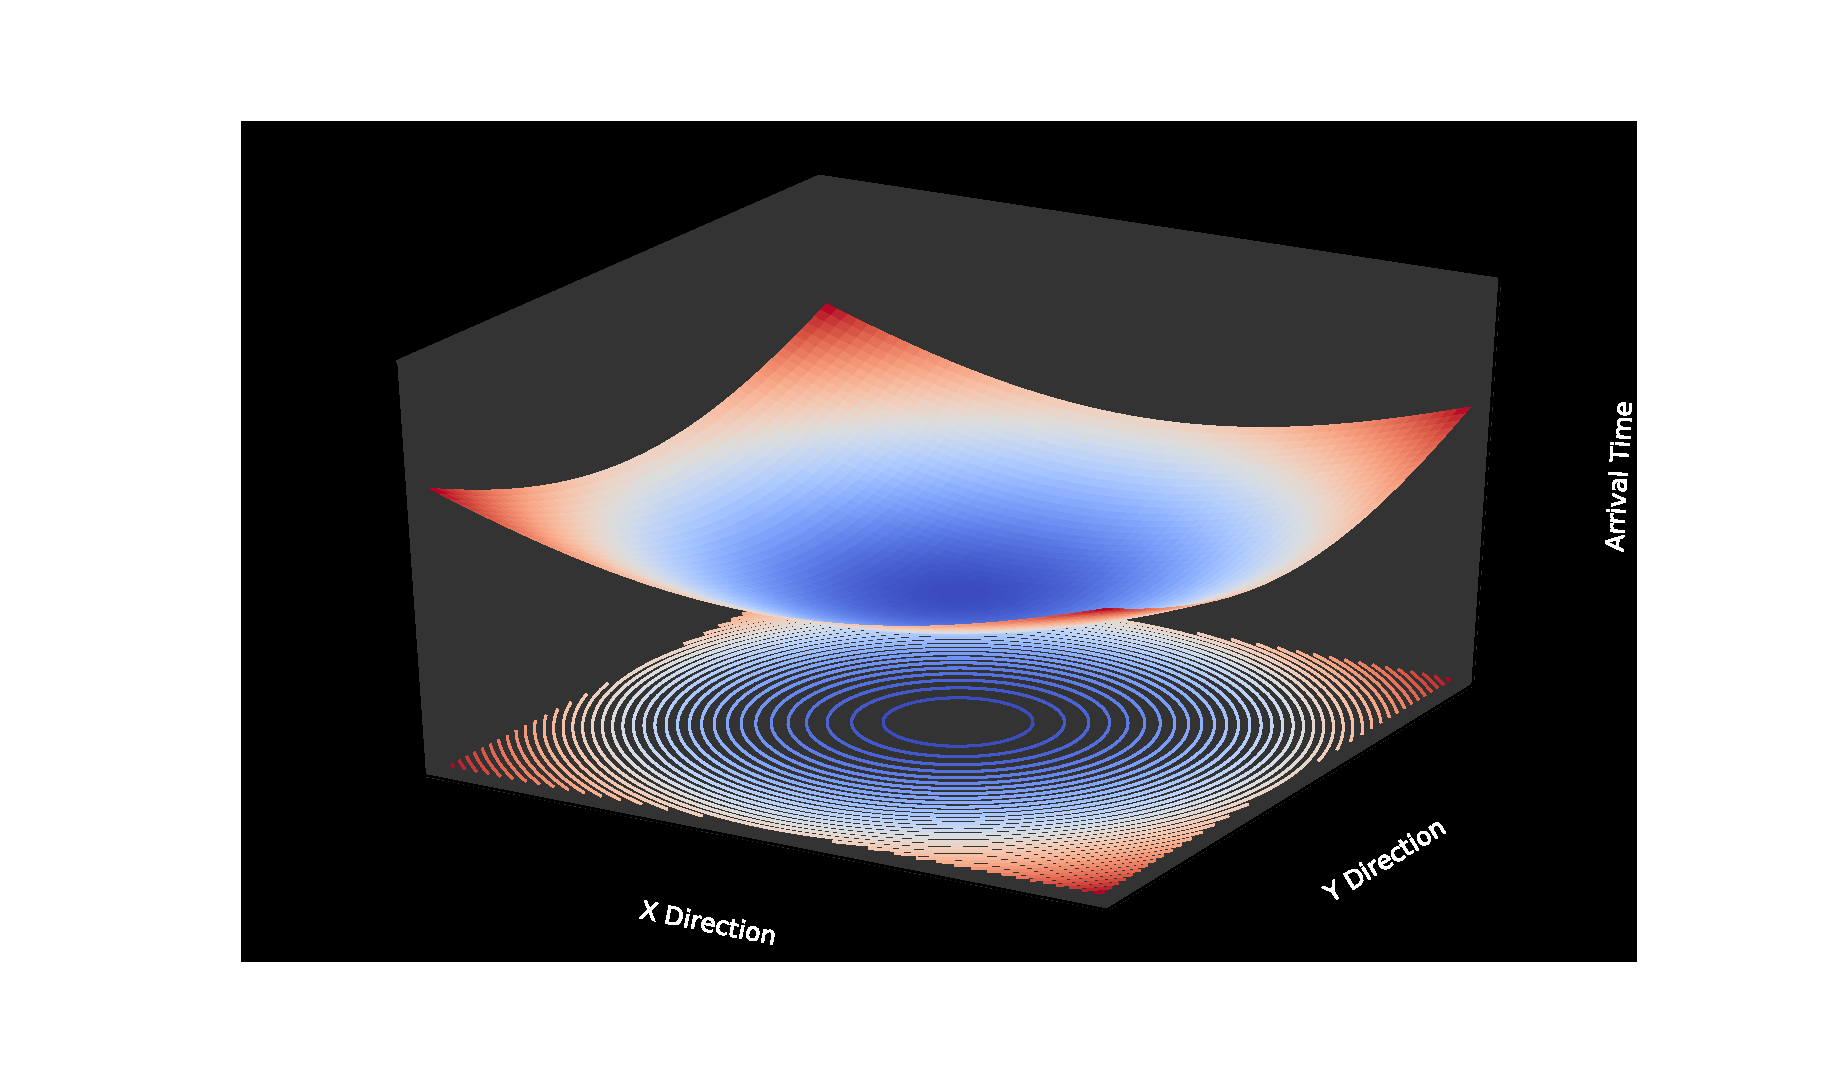
\includegraphics[width=\textwidth]{imgs/fig0}
\end{frame}

\begin{frame}
  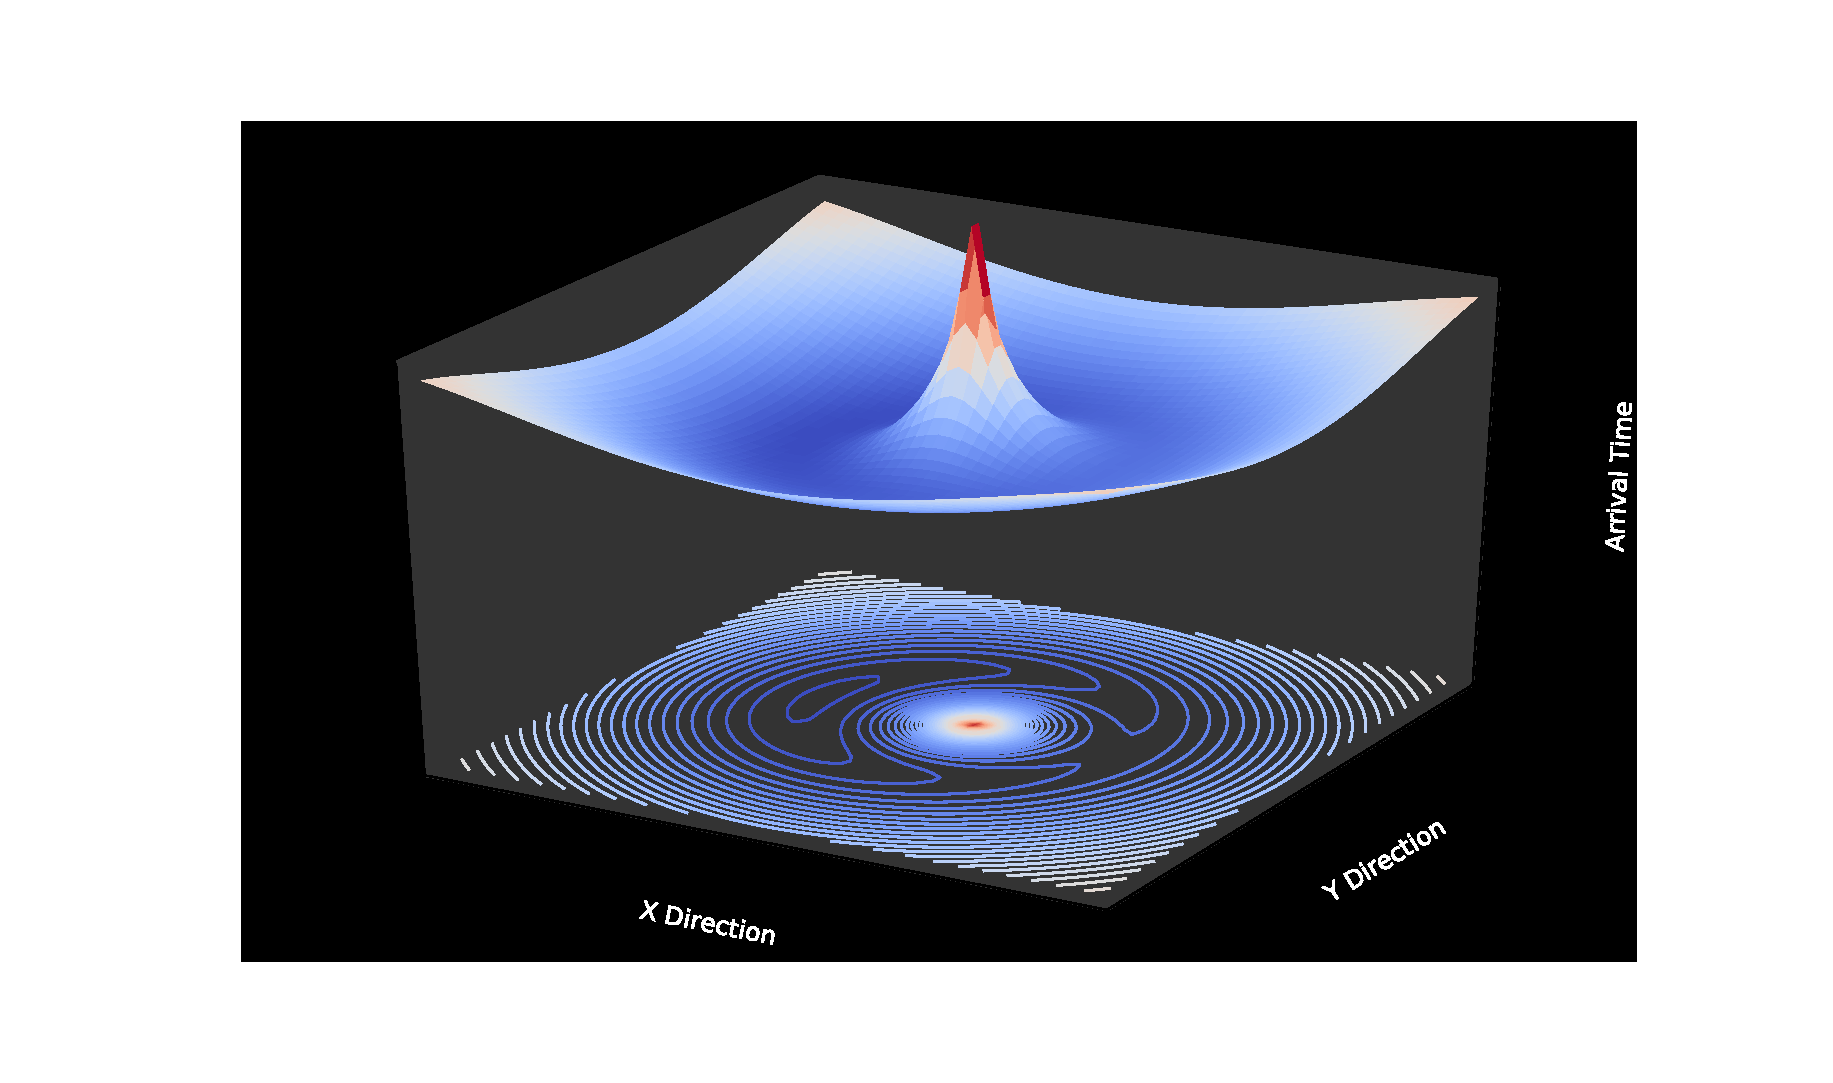
\includegraphics[width=\textwidth]{imgs/fig3}
\end{frame}}

%\begin{frame}
  %\includegraphics[width=\textwidth]{imgs/sl-3}
%\end{frame}
%
%\begin{frame}
  %\includegraphics[width=\textwidth]{imgs/real3}
%\end{frame}

\begin{frame}
  \begin{columns}[T]
    \begin{column}{5.5cm}
      \includegraphics[width=\textwidth]{imgs/sl-3}
    \end{column}
    \begin{column}{5.5cm}
      \includegraphics[width=\textwidth]{imgs/real3}
    \end{column}
  \end{columns}
\end{frame}

\begin{frame}
  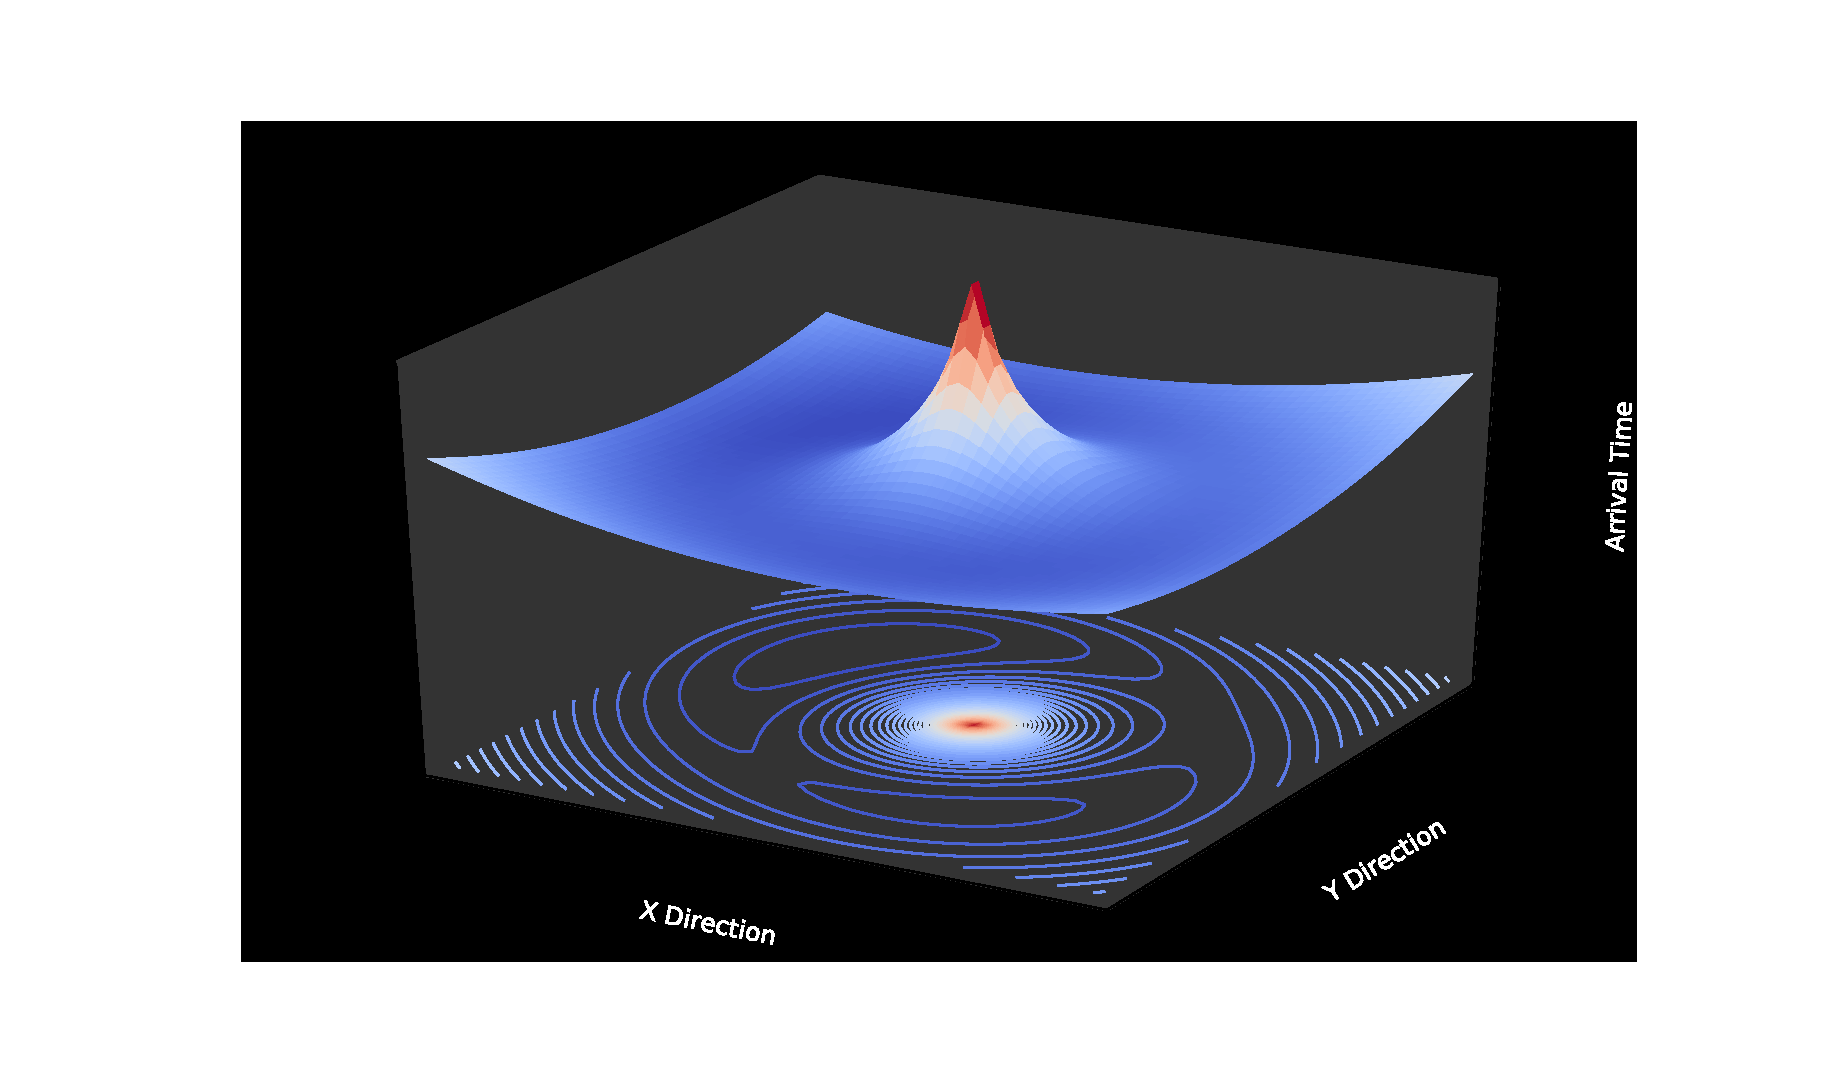
\includegraphics[width=\textwidth]{imgs/fig1}
\end{frame}

%\begin{frame}
  %\includegraphics[width=\textwidth]{imgs/sl-1}
%\end{frame}
%
%\begin{frame}
  %\includegraphics[width=\textwidth]{imgs/real1}
%\end{frame}

\begin{frame}
  \begin{columns}[T]
    \begin{column}{5.5cm}
      \includegraphics[width=\textwidth]{imgs/sl-1}
    \end{column}
    \begin{column}{5.5cm}
      \includegraphics[width=\textwidth]{imgs/real1}
    \end{column}
  \end{columns}
\end{frame}


\begin{frame}
  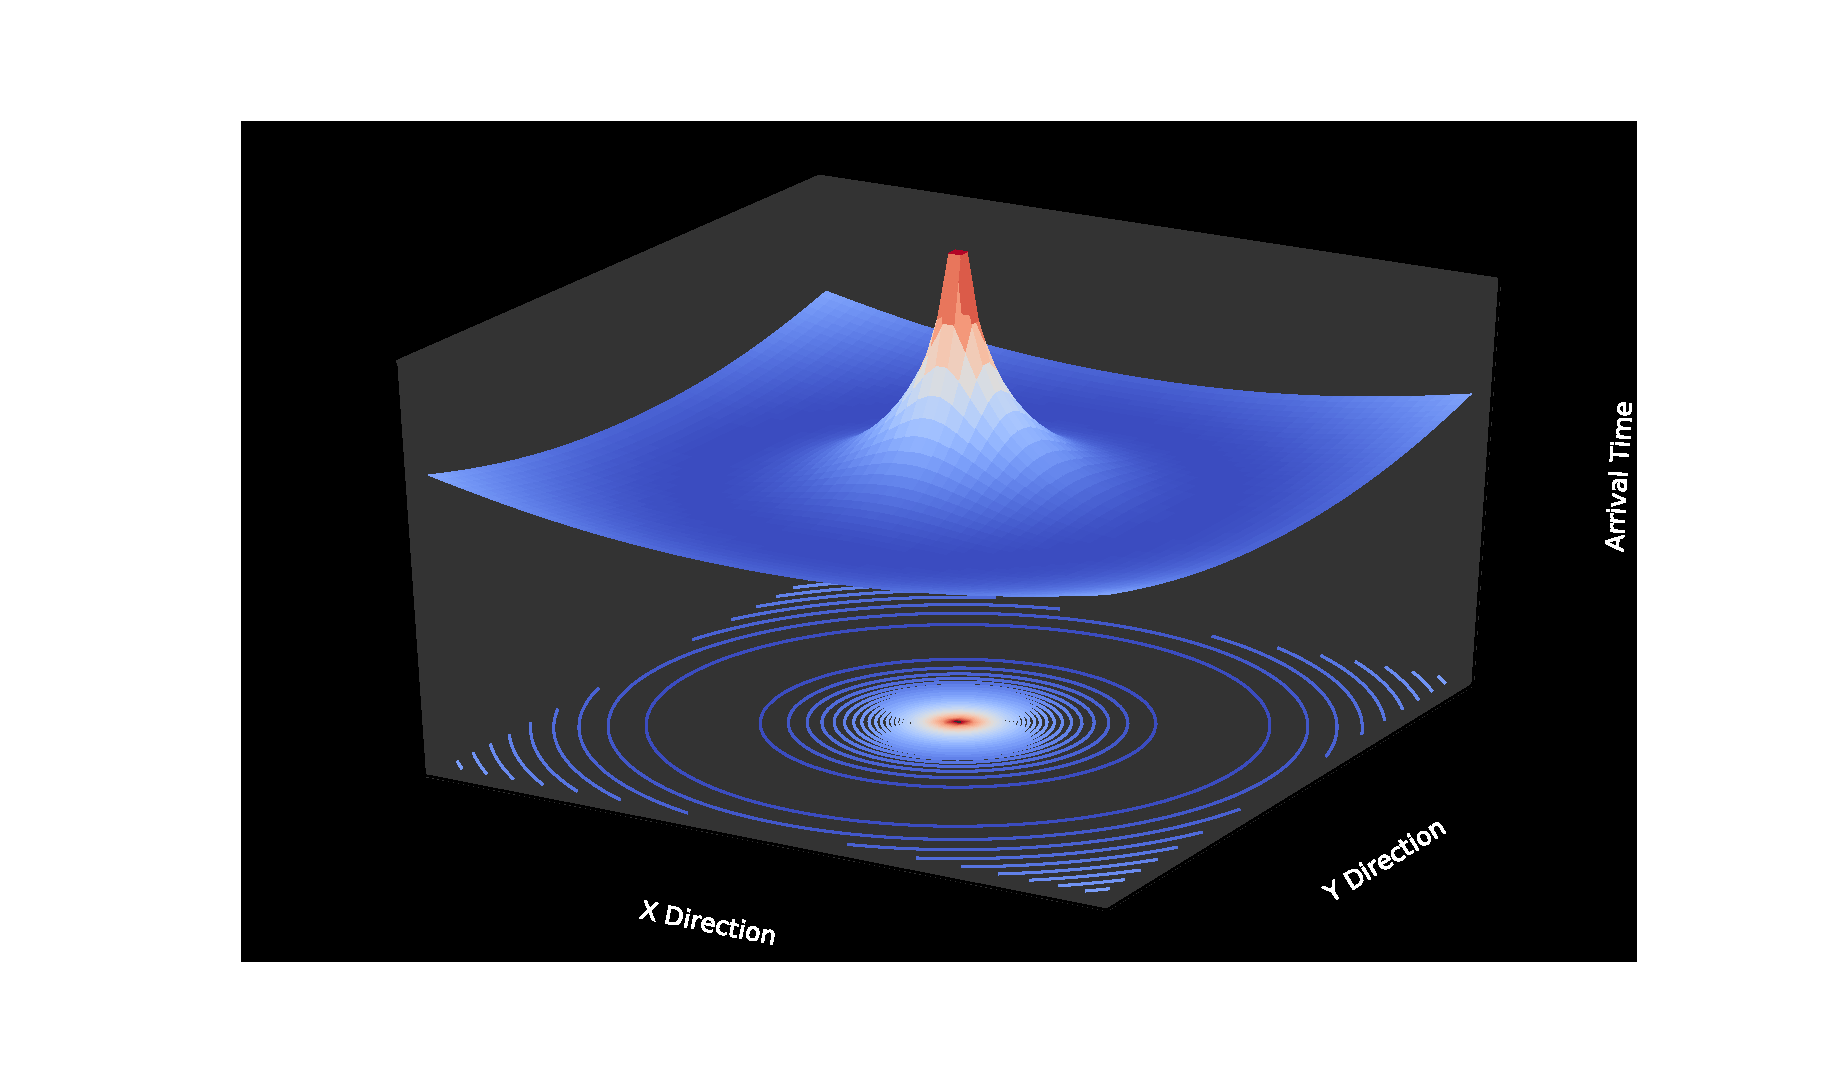
\includegraphics[width=\textwidth]{imgs/fig2}
\end{frame}

\begin{frame}
  \includegraphics[width=\textwidth]{imgs/einsteinring}
\end{frame}

\section{SpaghettiLens}
\subsection{Demonstration}

\begin{frame}
  \frametitle{SpaghettiLens}

  \begin{columns}[c]\begin{column}{0.55\textwidth}
    \begin{itemize}
    \item Extremal Points (Images)
    \item Self Intersecting Contour Lines
    \end{itemize}
    \url{http://mite.physik.uzh.ch/}

  \end{column}\begin{column}{0.44\textwidth}
    \includegraphics[width=\textwidth]{imgs/sled-1}
  \end{column}\end{columns}


\end{frame}

\subsection{Implementation}

\begin{frame}
  \frametitle{Implementation - Modules}
  \includegraphics[height=\textheight]{imgs/whole_setup}
\end{frame}

\begin{frame}
  \frametitle{Implementation - Data Flow}
  \includegraphics[width=\textwidth]{imgs/dataflow}
\end{frame}


\section{Involving Volunteers}
\subsection{Modeling Challenge}

\begin{frame}
  \frametitle{Modeling Challenge - Tests}
  \begin{itemize}
    \item some facts
    \item and the tests
  \end{itemize}
\end{frame}

\begin{frame}
  \frametitle{Results T1}
  \begin{table}\centering\begin{tabular}{llcc}\hline
 & & n & p \\
\hline
 N: & Total number of models & 119 & 1.00\\
\hline
 R1: & images approx. on right location & 110 & 0.92\\
 R2: & images with correct parity & 70 & 0.59\\
\hline
 E01: & inaccurate in arc & 21 & 0.18\\
 E02: & wrong parity in 3 img. conf. & 2 & 0.02\\
 E03: & identified 3 of 5 imgs. & 5 & 0.04\\
 E04: & modeled arc with single img. & 4 & 0.03\\
 E05: & $\pi$ rotated & 7 & 0.06\\
 E06: & $\pi$/2 rotated & 38 & 0.32\\
 E07: & missed faint img. & 1 & 0.01\\
 E08: & too many imgs in arc & 5 & 0.04\\
 E09: & missed double img & 3 & 0.03\\
 E10: & too many imgs. & 1 & 0.01\\
\hline

\end{tabular}\caption{T1 evaluation}\label{tab:stats}\end{table}
\end{frame}

\begin{frame}
  \frametitle{Results T2}
  \begin{columns}[c]\begin{column}{0.66\textwidth}
    \includegraphics[height=0.9\textheight]{imgs/eR_4}
  \end{column}\begin{column}{0.33\textwidth}
    {\color{red}XXX}
  \end{column}\end{columns}
\end{frame}


\subsection{Collaborative Modeling}

\section*{End}
\subsection*{Questions?}





\begin{frame}
  \frametitle{ttest}
  bla?\footcite{glass-jc}
  \transduration{1}
\end{frame}

\begin{frame}
  \frametitle{ttest}
  bla1\footcite{glass-jc}
\end{frame}

\appendix

\begin{frame}
  \frametitle{Appendix}
\end{frame}

\begin{frame}
\end{frame}


\end{document}